%%%%%
%%
%% Afstudeerverslag
%%
%% Version: v0.1
%% Authors: Iain Munro
%% Date: 18/02/2018
%%%%%

%Install packages using:
%sudo tlmgr install

% Available documentclass options:
%
%   <all `report` document class options, e.g.: `a5paper`>
%   withindex   - enables the index. New index entries can be added through `\index{my entry}`
%   glossary    - enables the glossary.
%   techreport  - typesets the thesis in the technical report format.
%   firstyr     - formats the document as a first-year report.
%   times       - uses the `Times` font.
%   backrefs    - add back references in the Bibliography section
%
% For more info see `README.md`
\documentclass[firstyr,a4paper,oneside]{cam-thesis}%withindex
\usepackage[dutch]{babel}
% Citations using numbers
\usepackage[numbers]{natbib}

\usepackage[utf8]{inputenc}

%APA norm
\usepackage{natbib}

%tables new lines
\usepackage{makecell}

%Set the title spacing correctly
\usepackage{titlesec}
\titlespacing{\chapter}{0pt}{0pt}{0pt}
\titlespacing{\section}{0pt}{0pt}{0pt}
\titlespacing{\subsection}{0pt}{0pt}{0pt}

% Copyright 2017 Sergei Tikhomirov, MIT License
% https://github.com/s-tikhomirov/solidity-latex-highlighting/

\usepackage{listings, xcolor}

\definecolor{verylightgray}{rgb}{.97,.97,.97}

\lstdefinelanguage{Solidity}{
	keywords=[1]{anonymous, assembly, assert, balance, break, call, callcode, case, catch, class, constant, continue, contract, debugger, default, delegatecall, delete, do, else, event, export, external, false, finally, for, function, gas, if, implements, import, in, indexed, instanceof, interface, internal, is, length, library, log0, log1, log2, log3, log4, memory, modifier, new, payable, pragma, private, protected, public, pure, push, require, return, returns, revert, selfdestruct, send, storage, struct, suicide, super, switch, then, this, throw, transfer, true, try, typeof, using, value, view, while, with, addmod, ecrecover, keccak256, mulmod, ripemd160, sha256, sha3}, % generic keywords including crypto operations
	keywordstyle=[1]\color{blue}\bfseries,
	keywords=[2]{address, bool, byte, bytes, bytes1, bytes2, bytes3, bytes4, bytes5, bytes6, bytes7, bytes8, bytes9, bytes10, bytes11, bytes12, bytes13, bytes14, bytes15, bytes16, bytes17, bytes18, bytes19, bytes20, bytes21, bytes22, bytes23, bytes24, bytes25, bytes26, bytes27, bytes28, bytes29, bytes30, bytes31, bytes32, enum, int, int8, int16, int24, int32, int40, int48, int56, int64, int72, int80, int88, int96, int104, int112, int120, int128, int136, int144, int152, int160, int168, int176, int184, int192, int200, int208, int216, int224, int232, int240, int248, int256, mapping, string, uint, uint8, uint16, uint24, uint32, uint40, uint48, uint56, uint64, uint72, uint80, uint88, uint96, uint104, uint112, uint120, uint128, uint136, uint144, uint152, uint160, uint168, uint176, uint184, uint192, uint200, uint208, uint216, uint224, uint232, uint240, uint248, uint256, var, void, ether, finney, szabo, wei, days, hours, minutes, seconds, weeks, years},	% types; money and time units
	keywordstyle=[2]\color{teal}\bfseries,
	keywords=[3]{block, blockhash, coinbase, difficulty, gaslimit, number, timestamp, msg, data, gas, sender, sig, value, now, tx, gasprice, origin},	% environment variables
	keywordstyle=[3]\color{violet}\bfseries,
	identifierstyle=\color{black},
	sensitive=false,
	comment=[l]{//},
	morecomment=[s]{/*}{*/},
	commentstyle=\color{gray}\ttfamily,
	stringstyle=\color{red}\ttfamily,
	morestring=[b]',
	morestring=[b]"
}

\lstset{
	language=Solidity,
	backgroundcolor=\color{verylightgray},
	extendedchars=true,
	basicstyle=\footnotesize\ttfamily,
	showstringspaces=false,
	showspaces=false,
	numbers=left,
	numberstyle=\footnotesize,
	numbersep=9pt,
	tabsize=2,
	breaklines=true,
	showtabs=false,
	captionpos=b
}

%Om de pagina margins etc te debuggen
%\usepackage{showframe}

\usepackage{pgfgantt}
\usepackage{rotating}
\usepackage[graphicx]{realboxes}

%%%%%%%%%%%%%%%%%%%%%%%%%%%%%%%%%%%%%%%%%%%%%%%%%%%%%%%%%%%%%%%%%%%%%%%%%%%%%%%%
%% Style (Changing the visual style of chapter headings and stuff.)
%%
\RequirePackage{titlesec}
% [Fixes issue #34 (see https://github.com/cambridge/thesis/issues/34). Solution from: http://tex.stackexchange.com/questions/299969/titlesec-loss-of-section-numbering-with-the-new-update-2016-03-15
\RequirePackage{etoolbox}
\makeatletter
\patchcmd{\ttlh@hang}{\parindent\z@}{\parindent\z@\leavevmode}{}{}
\patchcmd{\ttlh@hang}{\noindent}{}{}{}
\makeatother
% end of issue #34 fix]
\newcommand{\PreContentTitleFormat}{\titleformat{\chapter}[display]{\scshape\Large}
{\Large\filleft\MakeUppercase{\chaptertitlename} \Huge\thechapter}
{1ex}
{}
[\vspace{1ex}\titlerule]}
\newcommand{\ContentTitleFormat}{\titleformat{\chapter}[display]{\scshape\huge}
{\Large\filleft\MakeUppercase{\chaptertitlename} \Huge\thechapter}
{1ex}
{\titlerule\vspace{1ex}\filright}
[\vspace{1ex}\titlerule]}
\newcommand{\PostContentTitleFormat}{\PreContentTitleFormat}
\PreContentTitleFormat

%Om dubbelen legen pagina's weg te halen.
\let\cleardoublepage=\clearpage

%%%%%%%%%%%%%%%%%%%%%%%%%%%%%%%%%%%%%%%%%%%%%%%%%%%%%%%%%%%%%%%%%%%%%%%%%%%%%%%%
%% Thesis meta-information
%%

%% The title of the thesis:
\title{Afstudeerverslag}

%% The full name of the author (e.g.: James Smith):
\author{Calum Iain Munro}

%% College affiliation:
\college{Software Development, ICA, VT}

%% College shield [optional]:
\collegeshield{CollegeShields/ICA}

%% Submission date [optional]:
\submissiondate{June, 2018}

%% You can redefine the submission notice [optional]:
\submissionnotice{
HBO afstudeerverslag:\\
\textbf{Versie: 1 (definitief)}\\
\textbf{Datum: \today}\\
\\~\\
\textbf{Gegevens opdrachtgever:}\\
Bedrijf:			HeadForward B.V.\\
Contactpersonen:	Dani\"el Siahaya\\
\\~\\
\textbf{Gegevens opleiding:}\\
Opleiding: HBO bachelor Informatica\\
School: Hogeschool van Arnhem en Nijmegen\\
Begeleider:	Misja Nabben\\
Assessor: Rein Harle\\
\\~\\
\textbf{Gegevens opdrachtnemer:}\\
Teamlid: Calum Iain Munro (549288)\\
}

%% Declaration date:
\date{June, 2018}

%% PDF meta-info:
\subjectline{Afstudeerverslag}%Computer Science
\keywords{Afstudeerverslag Calum Iain Munro HAN}

% %%%%%%%%%%%%%%%%%%%%%%%%%%%%%%%%%%%%%%%%%%%%%%%%%%%%%%%%%%%%%%%%%%%%%%%%%%%%%%%%
% %% Abstract:
% %%

 \abstract{My abstract ...}

% %%%%%%%%%%%%%%%%%%%%%%%%%%%%%%%%%%%%%%%%%%%%%%%%%%%%%%%%%%%%%%%%%%%%%%%%%%%%%%%%
% %% Acknowledgements:
% %%
 \acknowledgements{My acknowledgements ...}

%%%%%%%%%%%%%%%%%%%%%%%%%%%%%%%%%%%%%%%%%%%%%%%%%%%%%%%%%%%%%%%%%%%%%%%%%%%%%%%%
%% Glossary [optional]:
%%
% \newglossaryentry{HOL}{
%     name=HOL,
%     description={Higher-order logic}
% }

%%%%%%%%%%%%%%%%%%%%%%%%%%%%%%%%%%%%%%%%%%%%%%%%%%%%%%%%%%%%%%%%%%%%%%%%%%%%%%%%
%% Inhoudsopgave:
%%
\begin{document}

\bibliographystyle{plainnat}

%%%%%%%%%%%%%%%%%%%%%%%%%%%%%%%%%%%%%%%%%%%%%%%%%%%%%%%%%%%%%%%%%%%%%%%%%%%%%%%%
%% Title page, abstract, declaration etc.:
%% -    the title page (is automatically omitted in the technical report mode).
\frontmatter{}

%Normale paragraven
\setlength{\parindent}{0em}
\setlength{\parskip}{1em}

%\chapter{Versiebeheer}
%\small
%\begin{center}
% \begin{tabular}{|c c c c|} 
% \hline
% Datum & Versie & Door wie & Aanpassing \\ [0.5ex] 
% \hline
% 12-03-2018 & v0  & Iain Munro & Eerste opzet \\
% \hline
%\end{tabular}
%\end{center}
%\end{small}


\chapter{Samenvatting}
Deze samenvatting beschrijft in hoofdpunten het afstudeertraject. Deze hoofdpunten zijn:
\begin{itemize} 
	\item De project omgeving
	\item De projectopdracht
	\item De belangrijkste behaalde resultaten
	\item De getrokken conclusies.
\end{itemize}
Het doel van deze samenvatting is om de belangrijkste onderdelen van dit afstudeerproject te tonen.

\section{Project omgeving}
Dit project heeft plaatsgevonden in het kantoor van HeadFWD, gevestigd aan het John M. Keynesplein 12-46 in Amsterdam. Het project is uitgevoerd door Iain Munro. Hij is hierbij begeleid door Daniël Siahaya, die met zijn rol als Product Owner in direct contact stond met de opdrachtgever, Allianz Group.

\section{Projectopdracht}
Tijdens de afstudeerstage bij HeadFWD is er onderzoek uitgevoerd naar de mogelijkheden om Blockchain technologie toe te passen voor het claimproces van verzekeringen bij Allianz Group.

\section{Belangrijkste Resultaten}
Het resultaat van dit afstudeeropdracht is vooral het Smart Contract geschreven in Solidity en het onderzoek naar de Blockchain technologie. Dit resultaat is terug te vinden in bijlagen \ref{appendix:contract}. Hiermee is de hoofdvraag van dit afstudeerproject: “Hoe is de blockchain technologie in te zetten om het claimproces van Allianz te automatiseren?” beantwoord.
\newpage

\section{Conclusies}
Na afloop van het project kunnen alle hoofdfunctionaliteiten van het claim systeem uitgevoerd worden. Gedurende het gehele project naar voren is gekomen dat de technieken die gebruikt worden met de Blockchain technologie daadwerkelijk functioneel zijn, maar niet altijd even goed meewerken.\par

Gesteld kan worden dat meer tijd nodig is om een goed werkend product neer te kunnen zetten. Verder is de conclusie die betrekking heeft tot mijn proces dat ik positieve feedback heb ontvangen van mijn bedrijfsbegeleider Daniël. Ik heb van een lastig project met veel onduidelijkheden en onstabiele techniek een goed resultaat geboekt en mijn proces juist en inzichtelijk uitgevoerd. Hieruit is te concluderen dat ik geslaagd ben in het behalen van het gewenste projectresultaat en de competenties vanuit school.

\chapter{Inleiding}
Voor u ligt het afstudeerverslag van Iain Munro, dat is geschreven naar aanleiding van het afstudeerproject dat loopt van 5 februari 2018 tot en met 29 juni 2018 (2017/2018 periode 3 & 4). De Afstudeeropdracht is uitgevoerd in opdracht van Allianz Group via het stagebedrijf HeadFWD. Deze opdracht bestond uit het ontwikkelen van een ’proof of concept’ voor de opdrachtgever, waarbij vooraf analyse en onderzoek werd uitgevoerd.
\par 
Het doel van dit verslag is om inzicht te geven over de inhoud, aanpak, verloop en resultaten van dit project. Het eerste gedeelte van dit verslag heeft betrekking op de context van het project. Hierna volgt de opdrachtomschrijving, waarin kort de opdracht en het uitgevoerde onderzoek worden beschreven. Aangezien dit al eerder uitgebreid is beschreven wordt hier alleen kort samengevat met een verwijzing naar het Plan van Aanpak.
\par
Vervolgens worden de gebruikte methoden en technieken besproken. Hierbij wordt voornamelijk gekeken naar de reden waarom deze technieken zijn gebruikt, en in hoeverre deze nuttig waren voor het project. Verder staat er een korte beschrijving van alle (tussen)resultaten van het project.
\par
In de procesbeschrijving worden de belangrijkste activiteiten en besluiten verantwoord. Hierbij wordt verwezen naar de verschillende competenties die de bekwaamheid aantonen van de afstudeerder als beginnend beroepsprofessional. Verder worden de opgeleverde resultaten en producten toegelicht. Hierdoor zou er een duidelijk beeld moeten ontstaan en zou het helder moeten zijn in hoeverre deze voldoen aan de gestelde eisen. Het volledige eindproduct is meegeleverd met dit document en een verwijzing is te vinden in de bijlagen.
\par
Dit verslag wordt afgerond met de conclusies en aanbevelingen. Hierin wordt teruggekoppeld naar de opdracht- en doelstelling van het project. De vraag “In hoeverre ben ik geslaagd in het gewenste projectresultaat en daarmee de doelstelling(en) van het project te behalen” wordt hier beantwoord, en de belangrijkste conclusies worden weergegeven. Op de momenten waar het gaat over mijn proces maak ik gebruik van de ik vorm, omdat dit gaat over mijn proces. Naar aanleiding van deze conclusies wordt er een aanbeveling gedaan voor eventuele vervolgacties of aandachtspunten voor het opgeleverde resultaat.
\par
Het einde van dit verslag bestaat uit een bronnenlijst waarbij de opgeleverde producten zoals het Plan van Aanpak, Onderzoeksverslag en Analyse documenten zijn meegeleverd met dit verslag. 

\chapter{Context}
Het afstudeerproject wordt uitgevoerd bij HeadFWD voor een van hun klanten, Allianz Group. HeadFWD is een consultancy bedrijf en ontwikkelt, beheert en host daarnaast maatwerk software en data- en integratie oplossingen \cite{pva}. 
\par
De Allianz Group is een Duitse verzekeringsmaatschappij\cite{pva} en heeft HeadFWD gevraagd om bepaalde bedrijfsprocessen te automatiseren, waaruit dit afstudeerproject is gevormd. Verdere details over de opdracht zijn beschreven in het volgende hoofdstuk. 
\par
De werkzaamheden voor afstudeeropdracht zijn bij HeadFWD op kantoor in Amsterdam uitgevoerd. Het project wordt full-time alleen uitgevoerd door Iain Munro onder begeleiding van Daniël Siahaya die de rol als productowner heeft vervuld.

\section{Begeleiders}
Voor dit afstudeerproject zijn er vanuit de Hogeschool Arnhem Nijmegen Misja Nabben als stagebegeleider aangesteld en Rein Harle als Assessor. Zie het Plan van Aanpak \cite{pva} voor de contactgegevens.
\chapter{Opdrachtomschrijving}
Zoals behandeld in het plan van aanpak verzekert de opdrachtgever, Allianz Group panden voor miljoenen. Zogenoemde co-insurance verzekeringen worden in de praktijk gedeeld met meerdere verzekeraars, om zo het risico te verspreiden.\par

Het probleem en ook gelijk de aanleiding voor dit project is dat het claimproces te veel tijd kost voordat deze wordt uitgekeerd naar de klant. Dit komt doordat het door verschillende bedrijven en hun handmatige bedrijfsprocessen gevalideerd moet worden. Hierdoor kan een claim vaak 3 maanden of langer duren voordat deze werkelijk wordt uitbetaald.

\section{Doelstelling}
De doelstelling van dit project is het versnellen van het claimproces. Zodat claims sneller uitbetaald worden. Om dit doel te bereiken wordt er een proof of concept (POC) ontwikkeld, waarin de nieuwe situatie wordt gedemonstreerd.

Om dit doel te bereiken is er eerst onderzoek uitgevoerd naar de blockchain technologie en de verschillende mogelijke oplossingen. Hoe ik tot deze vragen ben gekomen staat in mijn onderzoeksverslag\cite{onderzoeksverslag}. Verder is er analyse uitgevoerd om de requirements en use cases in kaart te brengen voor het proof of concept.

De subdoelstelling van dit afstudeerproject is kennis opbouwen over de blockchain en smart contract technologieën. Hiermee kunnen in vervolgprojecten of voor andere use cases hier gebruik van gemaakt kan worden.

\chapter{Methode}
Om het project kwalitatief goed uit te kunnen voeren is er gebruik gemaakt van verschillende methoden en technieken. Er is gezien de HBO vaardigheden competenties en kenmerken van het project gekozen voor een agile iteratieve projectmethodiek. Als projectmethodiek is er gekozen voor Kanban, die verder beschreven is in het plan van aanpak [PVA].\par
De reden voor deze aanpak is omdat hiermee werk gestructureerd opgesplitst, ingeschat, geprioriteerd en ingepland wordt in iteraties. Dit geeft de vereiste flexibiliteit om snel te kunnen schakelen bij aanpassingen of nieuwe requirements. Dit vereist het gebruik van experimentele software, materie en technologieën die nog niet bekend waren voordat dit project begon.\par
Deze praktische aanpak maakt het mogelijk dat bevindingen tijdens het onderzoeken naar een onderwerp gelijk gebruikt kunnen worden in een stuk ontwikkeling van het prototype (proof of concept). Verder is er voor Kanban gekozen omdat het project niet in teamverband wordt uitgevoerd. Kanban, in tegenstelling tot Scrum, vereist niet de teamvergaderingen die normaal gesproken nodig zijn als het project in teamverband wordt uitgevoerd (daily standups, retrospectives etc..).\par
Met de uitvoering van Kanban is er gekozen om gebruik te maken van het whiteboard op kantoor, zie figuur \ref{fig:kanbanbord}. Het bord bestaat uit vier kolommen: To Do, In Progress, Review en Done. Net als de bekende Scrum methodiek staat hier al het opgesplitste werk op, voor zowel de school als voor het stagebedrijf. Zo wordt alles eerst onder het kopje To Do gezet. Het werk wat een hoge prioriteit heeft, wordt bovenaan geplaatst. Wanneer ik begin met een nieuwe ticket dan wordt deze verplaatst naar de In Progress kolom. Op het moment dat ik het werk heb afgerond wordt deze eerst opgestuurd voor feedback en acceptatie. Dit gebeurt door de ticket in de review kolom te plaatsen.\par
\newpage

Zodra een ticket goedgekeurd is door de stakeholder, dan wordt het werk als klaar beschouwd. In het geval van het proof of concept onderzoek of analyse documenten, wordt deze review uitgevoerd door de productowner (Daniël Siahaya) of in sommige gevallen door de opdrachtgever (Allianz Group, Arjan Zaal). Het werk voor school wordt vanuit de review kolom naar To Do gezet nadat er feedback ontvangen is van de stagebegeleider en assessor.\par
Door deze aanpak is er één oogopslag duidelijk wat de huidige stand van zaken is. Dit geeft ook inzicht in het proces, want hierdoor wordt al snel duidelijk tegen het einde van een iteratie of er niet te veel nog staat bij de To Do of Doing kolom.\par
Hierdoor kan ik iedere iteratie nieuwe doelstellingen maken en controleren of het project nog op schema ligt. Op momenten dat dit niet zo is, kan er een juiste afstemming gemaakt worden. Deze retrospective \footnote{ https://www.atlassian.com/team-playbook/plays/retrospective} wordt uitgevoerd na iedere iteratie met de bedrijfsbegeleider, waar ik reflecteer op mijn eigen werkprocessen van die iteratie. Deze retrospective momenten hebben in het begin wat meer tijd gekost, maar met het verloop van het project zijn deze momenten steeds minder nodig. Na een iteratie wordt dan ook de resultaten of bevindingen van onderzoek behandeld en gekeken naar wat er te doen staat in de volgende iteratie. Om deze feedback loop zo kort mogelijk te houden is er gekozen voor 2 weken iteraties, zodat er voldoende tijd is om resultaten te boeken en voldoende feedback momenten zijn.
\begin{figure}[h]
    \begin{center}
        \includegraphics[width=\paperwidth-200]{images/kanbanbord}
        \caption{Foto genomen van het Kanban bord op 11-06-2018}
        \label{fig:kanbanbord}
    \end{center}
\end{figure}
\newpage

\section{Technieken}
Er zijn meerdere technieken gebruikt tijdens het project, waarvan een aantal die bekend zijn vanuit de studie. Om te beginnen is er een work breakdown structure gebruikt om werk op te splitsen en vervolgens op te schrijven op post-its op het kanban bord. Om te achterhalen wat de requirements, user stories en het minimum viable product zijn, is er analyse uitgevoerd en verbaal overleg uitgevoerd met de opdrachtgever en de product owner. Deze analyse is vastgelegd in een requirements document en specificeert op een gestructureerde en gestandaardiseerde manier door UML en C4 diagrammen te maken. Deze opgestelde eisen zijn gemaakt gedurende het software- ontwikkeltraject en vervolgens evalueert op basis van gebruikersbehoeften per user story deze door te nemen met de klant. (SD-1)\par
Voor het vermelden van de gebruikte bronnen is de APA richtlijnen gebruikt en tevens verplicht vanuit de HAN. Voor het indelen van de te maken producten en requirements is de MoSCoW-methode toegepast. Er wordt tijdens de ontwikkeling van het proof of concept gebruik gemaakt van GIT, versiebeheer systeem. Waarbij de GitFlow best practice is gebruikt om met iedere nieuwe feature een nieuwe git branch te maken en deze te mergen met een pull-request.\par
Verder is op basis van ontwerp meerdere werkende en betekenisvolle data-intensieve en gedistribueerde software systemen gerealiseerd. Zo is bij de ontwikkeling van het Smart Contract  rekening gehouden met hergebruik, het verminderen van complexiteit en onderhoudbaarheid. Deze code bevat ook de core business rules en is daarom ge-unit test.\par
Er is geen gebruik gemaakt van continuous integration of deployment gezien de tijdsdruk en het feit dat het een prototype is dat na dit afstudeerproject niet verder gebruikt zou worden.\par
Tijdens het onderzoek zijn er prototyping en experimenten uitgevoerd naast literatuuronderzoek. Zo is voor de Blockchain technologie kleinschalig, systematisch en methodisch onderzoek uitgevoerd. De bevindingen en conclusies hieruit hebben geholpen om bepaalde besluiten in het project te onderbouwen.\par
Er is geen digitaal Kanban bord gebruikt zoals Trello of Jira, omdat het fysieke bord voldoende is geweest. Dit is mede mogelijk omdat ik iedere dag op kantoor ben en niemand anders op afstand hier naar hoeft te kijken.

\subsection{C4 framework}
Voor het modelleren van de architectuur is er gekozen voor de Simon Brown’s C4 Framework. Deze techniek is mij geleerd tijdens het Advanced Software Development semester. De reden hiervoor was dat door de gekozen agile projectaanpak, software design niet met een heavy upfront design wordt uitgevoerd. Met een agile aanpak wordt bijvoorbeeld UML vooral gebruikt om informele aantekening te maken die bestaan uit vierkanten en lijnen om een verbaal verhaal duidelijk te krijgen. Het probleem hiermee alleen is dat dit niet heel inzichtelijk is of het waard is om in een document mee te nemen.\par
Door het gebruik van C4 framework heb ik een formele manier van communicatie waarmee ik aan de verschillende stakeholders de software architectuur kan uitleggen. Hiermee kan ik agile ontwikkelen en tegelijkertijd de competenties SD-2 en SD-3 vanuit school aantonen en de architectuur duidelijk krijgen. Dit doet C4 door 4 verschillende diagrammen te ontwikkelen met variërende niveaus van abstractie.\par
Deze argumentatie is hetgeen wat mij is geleerd tijdens de SWA lessen en is terug te vinden in slide 11 van de Software Architecture Course: Simon Brown’s C4 Framework.
\chapter{Process en resultaten}
In dit hoofdstuk beschrijf ik het proces en de resultaten van het afstudeerproject. Bij afwijkingen van het originele plan dat beschreven in het Plan Van Aanpak is dit beargumenteerd. Verder wordt er in dit hoofdstuk alleen het proces en de resultaten geconstateerd. Reflectie hierop en mijn keuzes worden in een volgend hoofdstuk beschreven en in dit hoofdstuk constateer ik alleen wat er is gebeurd.

\section{Verloop van het project}
Om het verloop van het project gestructureerd te verwoorden, is het project te verdelen in 4 fases: Initiatie fase, definitie fase, analyse en realisatie fase en afronding fase. Dit zijn ook de fases die opgenomen zijn in de planning in het plan van aanpak en zijn in de onderstaande subparagrafen op chronologische volgorde beschreven.\par

Door de agile aanpak is in derde fase er beide analyse en realisatie tegelijkertijd uitgevoerd.  De gekozen Kanban agile methode laat dit ook toe. De reden hiervoor is om risico’s van het project te verminderen door de software, het onderzoek en enige analyse tegelijkertijd stukje voor stukje uit te voeren in iteraties \footnote{https://www.twynstraguddekennisbank.nl/projectmanagement/faseer-het-project}.

\subsection{Fase: Initiatieffase (iteratie 0)}
In deze eerste fase is het doel om een gelijk beeld van het project te verkrijgen van alle betrokkenen aan het project en hiermee goedkeuring te krijgen om het project te starten. Dit is gedaan door de stand van zaken vast te stellen en onderzoek te doen naar de aanleiding en doelstelling van het project.\par

Deze fase is samen met de definitiefase uitgevoerd waar verdere analyse is gedaan naar het te ontwikkelen product. Dit is gedocumenteerd in het Plan Van Aanpak waarin het beoogde projectresultaat in termen van: randvoorwaarden, functionele en operationele prestaties, eisen, wensen en projectgrenzen duidelijk wordt. Een planning in de vorm van een GANTT chart met daarin de deadlines die vanuit school bekend zijn, geeft een beeld voor de komende fases.
\newpage

\subsection{Fase 2: Definitiefase (iteratie 0 - 1)}
In de tweede fase is er verder gekeken naar het te ontwikkelen product. In deze fase is het Plan van Aanpak verder afgerond en vervolgens goedgekeurd, door zowel de stagebegeleider en assessor als de bedrijfsbegeleider. De ontwikkelmethode, Kanban is gekozen en de planning voor de aankomende realisatie- en analysefase zijn opgesplitst in 7 iteraties van 2 weken. Daarbij wordt per iteratie gekeken naar wat er nodig is aan werk voor de komende 2 weken.\par

Om te beginnen is het duidelijk dat er een onderzoek gestart moet worden. De aanleiding hiervoor is dat het doel van het proof of concept moet aantonen dat het elektronische claim systeem use case van Allianz met de Blockchain Technologie geautomatiseerd kan worden.\par

Omdat ik zelf nog niet bekend ben met de Blockchain Technologie en het duidelijk is dat er in een later stadium een geïnformeerd besluit gemaakt over moet worden, is het duidelijk dat de eerste iteratie zich vooral bezighoudt met een algemeen onderzoek naar de Blockchain Technologie. Hiermee is de definitiefase afgerond en begint de analyse / realisatie fase. 

\subsection{Fase 3: Analyse / Realisatie Fase (Iteraties 1 - 5)}
Er is tijdens deze fase meerdere malen analyse en realisatie uitgevoerd. In de onderstaande subparagrafen beschrijf ik per iteratie hoe het proces is gelopen en waar aan gewerkt is. De grootste afwijking met het originele plan, in het plan van aanpak is het opsplitsen van de resultaten in het onderzoeksverslag dat bestaat uit een literatuuronderzoek, analyse en het proof of concept experiment. Dit wordt gedaan na het ontvangen van de feedback op de 80\% versie en om verwarring te vermijden wordt er in het proces hieronder verwezen naar de namen van de losse documenten die aan het einde van het project met dit afstudeerverslag zijn meegeleverd.
\newpage

\subsubsection{Iteratie 1 - Onderzoek naar Blockchain en huidige proces}
In de eerste iteratie is er gekeken naar hoe het huidige claim proces werkt. Deze analyse vult de analyse die is gestart voor het Plan van Aanpak aan met gesprekken met de opdrachtgever Allianz Group en de Product Owner. Uit deze analyse zijn requirements opgesteld en user stories en actoren van het te ontwikkelen proof of concept gedocumenteerd in het Software Architecture Document. (SD-1, SD-2)\par

Daarnaast is er een literatuuronderzoek uitgevoerd naar een technische basis termen rondom de blockchain-technologie en gerelateerde onderwerpen. Dit is gedaan om een aantal basis technische termen in cryptografie, blockchain-technologie en gerelateerde onderwerpen duidelijk te krijgen. Hiermee weet ik waar ik het over heb wanneer het proof of concept in vervolg iteraties behandeld wordt.\par

De focus is met name de manier waarop de blockchain gebruikt zou kunnen worden voor het doeleinde van de klant. Tijdens de eerste week is al snel duidelijk dat er verschillende types Blockchains zijn: Consortium, Privé en openbaar, en die zijn vervolgens onderzocht. (SD-7)
\newpage
\subsubsection{Iteratie 2 - Onderzoek naar de architectuur van de blockchain en smart contracts}
Tijdens de tweede iteratie is er verder onderzoek uitgevoerd naar de blockchain technologie en is het uitgebreid naar Smart Contracts en de blockchain zijn architectuur. Dit allemaal om duidelijk te krijgen hoe hiermee een gedecentraliseerde blockchain applicatie (Dapps \footnote{https://en.wikipedia.org/wiki/Decentralized\_application}) ontwikkeld zou kunnen worden.\par

Verder is het onderzoek aangevuld door bij het onderzoek naar de verschillende types blockchain te kijken wat handig is voor het proof of concept en welke populaire blockchain projecten een gedecentraliseerde applicatie op gebouwd zou kunnen worden. (SD-7)\par

Tijdens deze iteratie is de analyse naar welke factoren in het eindproduct verwerkt moet worden afgerond en vervolgens goedgekeurd door zowel de klant als de product owner. Dit is gedaan door de scope van het proof of concept met de MoSCoW analyse te definiëren.\par

Hieruit is gekozen dat de Must Haves betrekking hebben op het registeren van Claim aanvraag. Deze ziet op het moment dat iedere verzekeraar hierop zijn stem heeft ingevoerd of de claim geaccepteerd of geweigerd wordt. Verder was een Must Have dat dit allemaal door Blockchain transacties inzichtelijk en controleerbaar moet zijn voor iedere gebruiker van het systeem. Op het moment dat dit niet mogelijk is dan heeft het proof of concept een negatiever resultaat voor Allianz, want het doel was zonder een centraal punt alle transacties gevalideerd kunnen worden.\par

Should haves waren bijvoorbeeld om het werk te verminderen dat claim aanvragen met een bedrag onder 1000 euro en het type diefstal automatisch geaccepteerd zouden worden, mits hier voldoende tijd voor is. Daarnaast zijn functionaliteiten zoals het kunnen inloggen met een gebruikersnaam en wachtwoord opgenomen. De Could Haves, de factoren die een leuke toevoeging zouden zijn wanneer er voldoende tijd over is maar dat helaas niet het geval is, is dat polissen en nieuwe makelaars geregistreerd kunnen worden. (SD-1)\par

Daarnaast is in eerste instantie het plan dat het proof of concept gebruik zou maken van het bestaande E-ABS systeem. Na overleg met de stakeholders is duidelijk geworden in deze iteratie dat dit niet het doel is en dat het proof of concept alleen moet aantonen dat de use cases mogelijk zijn met de Blockchain technologie. Dit is ook gelijk een constraint waardoor er tijdens dit project niet gekeken hoeft te worden naar andere methodes dan de blockchain. Dit zou eventueel in een vervolgactie opgenomen kunnen worden.
\newpage
\subsubsection{Iteratie 3 - Analyse + Realisatie fase}
Het onderzoek naar de blockchain is in iteratie 3 afgerond. Er is voldoende informatie om een geïnformeerd besluit te maken op de juiste oplossingsrichting voor de blockchain technologie. \par

Tijdens deze iteratie en komende iteraties zijn Software Architecturele besluiten gemaakt met een techniek die mij is geleerd tijdens de Software Architectuur lessen in het ASD semester. De techniek houdt in dat de requirements die invloed hebben op de architectuur en andere invloeden, zogenaamde decision forces, opgeschreven en meegenomen worden met een architecturaal besluit. Deze decision forces zijn samen met de product owner opgesteld en met ieder oplossingsrichting meegenomen. (SD-2, SD-3)\par

In deze iteratie gaat het vooral om het besluit van Blockchain framework waarop het proof of concept opgebouwd zou worden. Door het onderzoek naar dit onderwerp in vorige iteraties kan hier vrij snel een besluit opgenomen worden. Het type blockchain dat handig is voor het proof of concept is al bekend: consortium. Hierin is er maar een blockchain technologie die voldoende functionaliteit en documentatie biedt om het proof of concept te bouwen.\par

Voor het modelleren van de architectuur is er gekozen voor de Simon Brown’s C4 Framework. Hier is in deze iteratie een start mee gemaakt waarmee ik 4 verschillende diagrammen kon ontwikkelen met variërende niveaus van abstractie.\par

Naast alle analyse is er ook een stuk software ontwikkeld in deze iteratie. Dit is namelijk het smart contract geschreven in Solidity waarmee de core functionaliteiten en business rules in zijn opgenomen. Zie bijlage A die in de eindfase alle belangrijke requirements R2, R3, R4, R6, R7, R8, R9, R10, R11, R13 en R14 opneemt en wordt uitgevoerd in de blockchain. Deze zijn vervolgens ge-unittest (SD-4, SD-5, SD-6, SD-8).\par

Tijdens de retrospective van deze iteratie is er besloten om de laatste twee iteraties meer focus te zetten op het bereiken van resultaten van het proof of concept.

\newpage
\subsubsection{Iteratie 4 - Analyse + Realisatie fase}
Tijdens de vierde iteratie is het smart contract verder ontwikkeld. Hierbij zijn functionaliteiten zoals het automatisch accepteren van een claim geïmplementeerd. Het probleem hiermee is alleen dat dit nog niet toegankelijk is voor een eindgebruiker. \par

Daarnaast wordt duidelijk vanuit Allianz dat een nieuwe requirement (R1) gebruikers de mogelijkheid moet geven om in te kunnen loggen op het systeem via een webapplicatie. Daarom is er in deze iteratie besloten om te werken aan een simpele web api met gebruiker niveaus, zodat het smart contract in een later stadium gebruikt kan worden door een Grafische gebruikersinterface. (SD-1, SD-4, SD-6, SD-8)\par

Zodoende is er tijdens deze fase gekeken naar een geschikte back-end framework. Hierbij is vooral rekening gehouden met het feit dat er een Blockchain API beschikbaar moet zijn waarmee functies binnen het smart contract aangeroepen kunnen worden. Een ander belangrijk decision force voor dit besluit, is de bekendheid met het framework en taal, om zo de ontwikkelingskosten lager te houden. Hieruit is het Sails JS framework gekozen in combinatie met Angular doordat het geschreven is in Javascript die mogelijkheid biedt om gebruik te maken van de officiële Ethereum JavaScript API, Web3. \par

In deze iteratie is de software architectuur bijgewerkt met de nieuwe besluiten (SD-3). Een ander besluit wordt gemaakt op het moment dat ik erachter kom dat het itereren door een lijst van objecten, zoals een lijst van claims in een smart contract niet mogelijk is. De oplossing hiervoor is het gebruik van een database die op basis van events de aggregatie van data in transacties toegankelijk maakt. Dit besluit is ook met decision forces besloten en doordat er een link naar de transactie (etherscan.io) blijft binnen de blockchain kan de verificatie en validatie uitgevoerd worden.

\subsubsection{Iteratie 5 - Realisatie fase}
In de vijfde iteratie is de api verder ontwikkeld. Om requirement R15 te vervullen is er deze iteratie ook een webapplicatie gemaakt in Angular. Deze applicatie biedt een simpele gebruikersinterface, waarop verschillende gebruikers kunnen inloggen en via web interface van de web-api gebruik maken en daarmee functies aanroepen in het smart contract. Deze iteratie is er vooral vol ontwikkeld aan het de backend en de front-end applicatie om zoveel mogelijk functionaliteiten te realiseren.\par

Gezien de beperkte tijd en de hoeveelheid werk zijn er een aantal besluiten gemaakt om het werk te verminderen. Zo is er het besluit genomen om het authenticatie gedeelte van de applicatie door Firebase te laten gebeuren. Aangezien dit niet het primaire doel is van het proof of concept en er al gebruik wordt gemaakt van Firebase.

\subsection{Fase 4: Afrondingsfase (Iteraties 6 - 7)}
De nazorg van dit project betreft eigenlijk alleen het afronden van documenten. Deze fase bevat ook een tussentijdse beoordeling van school, waaruit feedback is ontvangen om het grote onderzoeksverslag op te splitsen in losse documenten.

Verder is er tijdens deze fase gewerkt aan het afstudeerverslag wat u nu leest en zijn de bevindingen en conclusies uit het proof of concept op zijn geschreven in het proof of concept document.

\section{Resultaten en Producten}
Uit het proof of concept is gebleken dat het mogelijk is om het claimproces met de blockchain te automatiseren.\par
Het resultaat van dit afstudeeropdracht is vooral het Smart Contract geschreven in Solidity en het onderzoek naar de Blockchain technologie. Hiermee is de hoofdvraag van dit afstudeerproject: “Hoe is de blockchain technologie in te zetten om het claimproces van Allianz te automatiseren?” beantwoord.\par

De back-end en front-end code die er naast is ontwikkeld om het smart contract toegankelijk te maken, toont dat de volledige use cases van Allianz opgelost kunnen worden. De twee belangrijkste elementen van het proof of concept is dat nieuwe claims veilig geregistreerd worden in het smart contract op de blockchain. Met een wijziging van deze data is dit traceerbaar met een transactiecode. Dit is te zien in de onderstaande screenshot van de web applicatie, waar op het moment dat je op de transactiecode of verwerkingscode klikt je naar een externe derde website gaat die de transactie van data valideert in de blockchain.
\begin{figure}[h]
    \begin{center}
        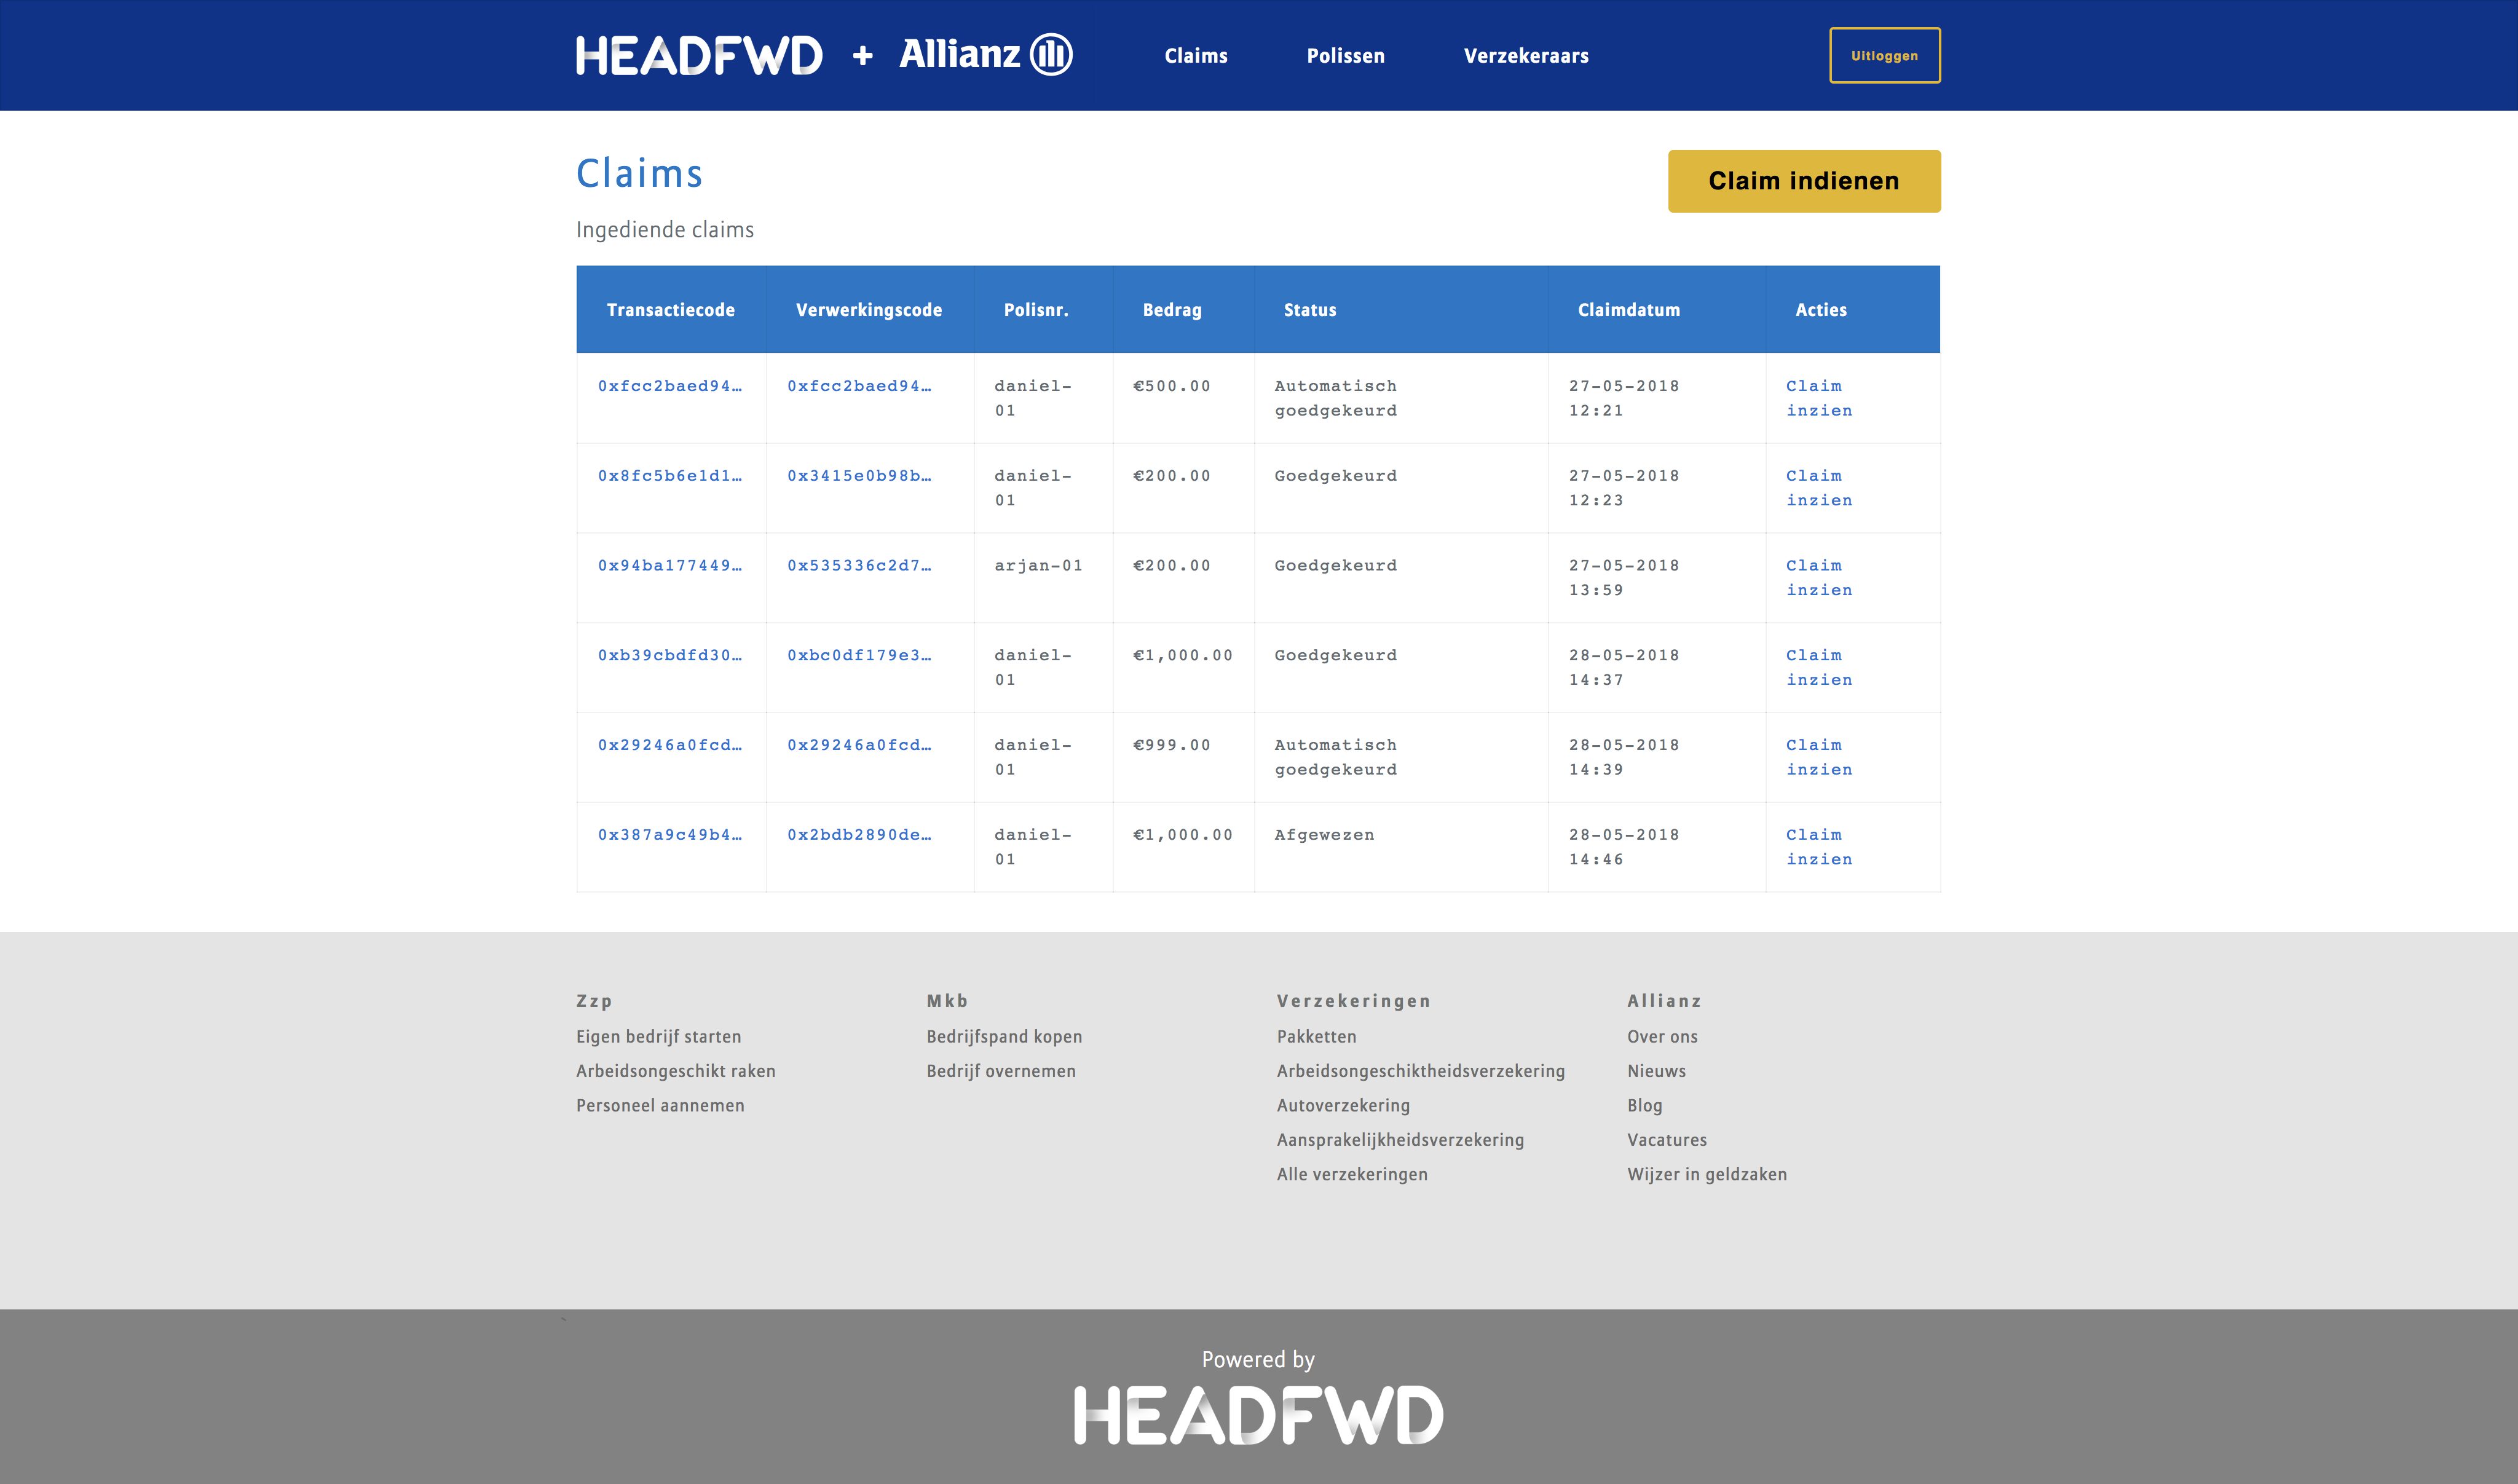
\includegraphics[width=\paperwidth-200]{images/claim-list}
        \caption{Foto van de user interface waar een lijst aan claims te zien is}
        \label{fig:claim-list}
    \end{center}
\end{figure}
Alle musts en zelf een aantals coulds uit de MoScow analyse zijn gerealiseerd. Zo kan bijvoorbeeld ingesteld worden dat om een bepaald claimbedrag een claim automatisch geaccepteerd wordt. Maar deze berekening wordt door iedere lid van het netwerk uitgevoerd.
\chapter{Conclusie \& Aanbevelingen}
In dit hoofdstuk kan aan de hand van dit gehele project de vraag “In hoeverre ben ik geslaagd in het gewenste projectresultaat en daarmee de doelstelling(en) van het project te behalen” worden beantwoord en de belangrijkste conclusies getrokken worden.

Het claimproces van co-insured verzekeringen duurt te lang. Het doel is om aan te tonen dat met de recent opkomende blockchain technologie bestaande bedrijfsprocessen geautomatiseerd kunnen worden. Het resultaat is de responstijd van een claim te verminderen en dit aan te tonen met een proof of concept.

Na afloop van het project kunnen alle hoofdfunctionaliteiten van het claim systeem uitgevoerd worden. Hieruit kan geconcludeerd worden dat de doelstelling van het project is behaald. Het proof of concept is in week 23 gepresenteerd aan de opdrachtgever, Allianz waarop positieve feedback is ontvangen.

Gedurende het gehele project is naar voren gekomen dat de technieken die gebruikt worden met de Blockchain technologie daadwerkelijk functioneel zijn, maar niet altijd even goed meewerken. Het kost veel tijd en uitzoekwerk en het grootste knelpunt zit voornamelijk in de documentatie en support om een gedecentraliseerde blockchain applicatie te realiseren.

Gesteld kan worden dat meer tijd nodig is om een goed werkend product neer te kunnen zetten. De API van de Blockchain verandert ook nog steeds en de applicatie die 2 weken geleden was ontwikkeld, is nu al niet meer compatible met de laatste versie van Ethereum. Hieruit kan ook geconcludeerd worden dat de techniek nog te nieuw is voor functioneel gebruik.

Verder is de conclusie die betrekking heeft tot mijn proces dat ik positieve feedback heb ontvangen van mijn bedrijfsbegeleider Daniël. Ik heb van een lastig project met veel onduidelijkheden en onstabiele techniek een goed resultaat geboekt en mijn proces juist en inzichtelijk uitgevoerd. Hieruit is te concluderen dat ik geslaagd ben in het behalen van het gewenste projectresultaat en de competenties vanuit school. 

\subsection{Aanbeveling}
Aan de hand van de bovenstaande conclusies kan er een aanbeveling gedaan worden. Gezien het feit dat na bijna zes maanden nog geen stabiel prototype gepresenteerd kan worden aan de opdrachtgever, is het aan te raden om dit door te ontwikkelen. Waar tijdens dit project niet naar gekeken hoeft te worden, is het gebruik van andere methodes dan de blockchain. Dit zou eventueel in een vervolgactie opgenomen kunnen worden.
\chapter{Reflectie}
In dit hoofdstuk reflecteer ik op mijn beroepsmatig handelen in het afstudeerproject. Deze reflectie voer ik uit aan de hand van situatiebeschrijvingen die volgens de STARRT methode zijn uitgewerkt. Deze situatiebeschrijvingen zijn opgesteld in het kader van:
\begin{itemize} 
	\item Mijn werkwijze en gemaakte keuzes ten aanzien van de projectuitvoering;
	\item Het toegepaste theoretisch kader;
	\item Het resultaat en de consequenties van het resultaat voor de organisatie.
\end{itemize}
Deze reflectie wordt gestructureerd gedaan op 4 kritische situaties in de volgende situatiebeschrijving zijn volgens de STARRT methode.

\section{Situatiebeschrijvingen}

\subsection{Projectaanpak keuze}
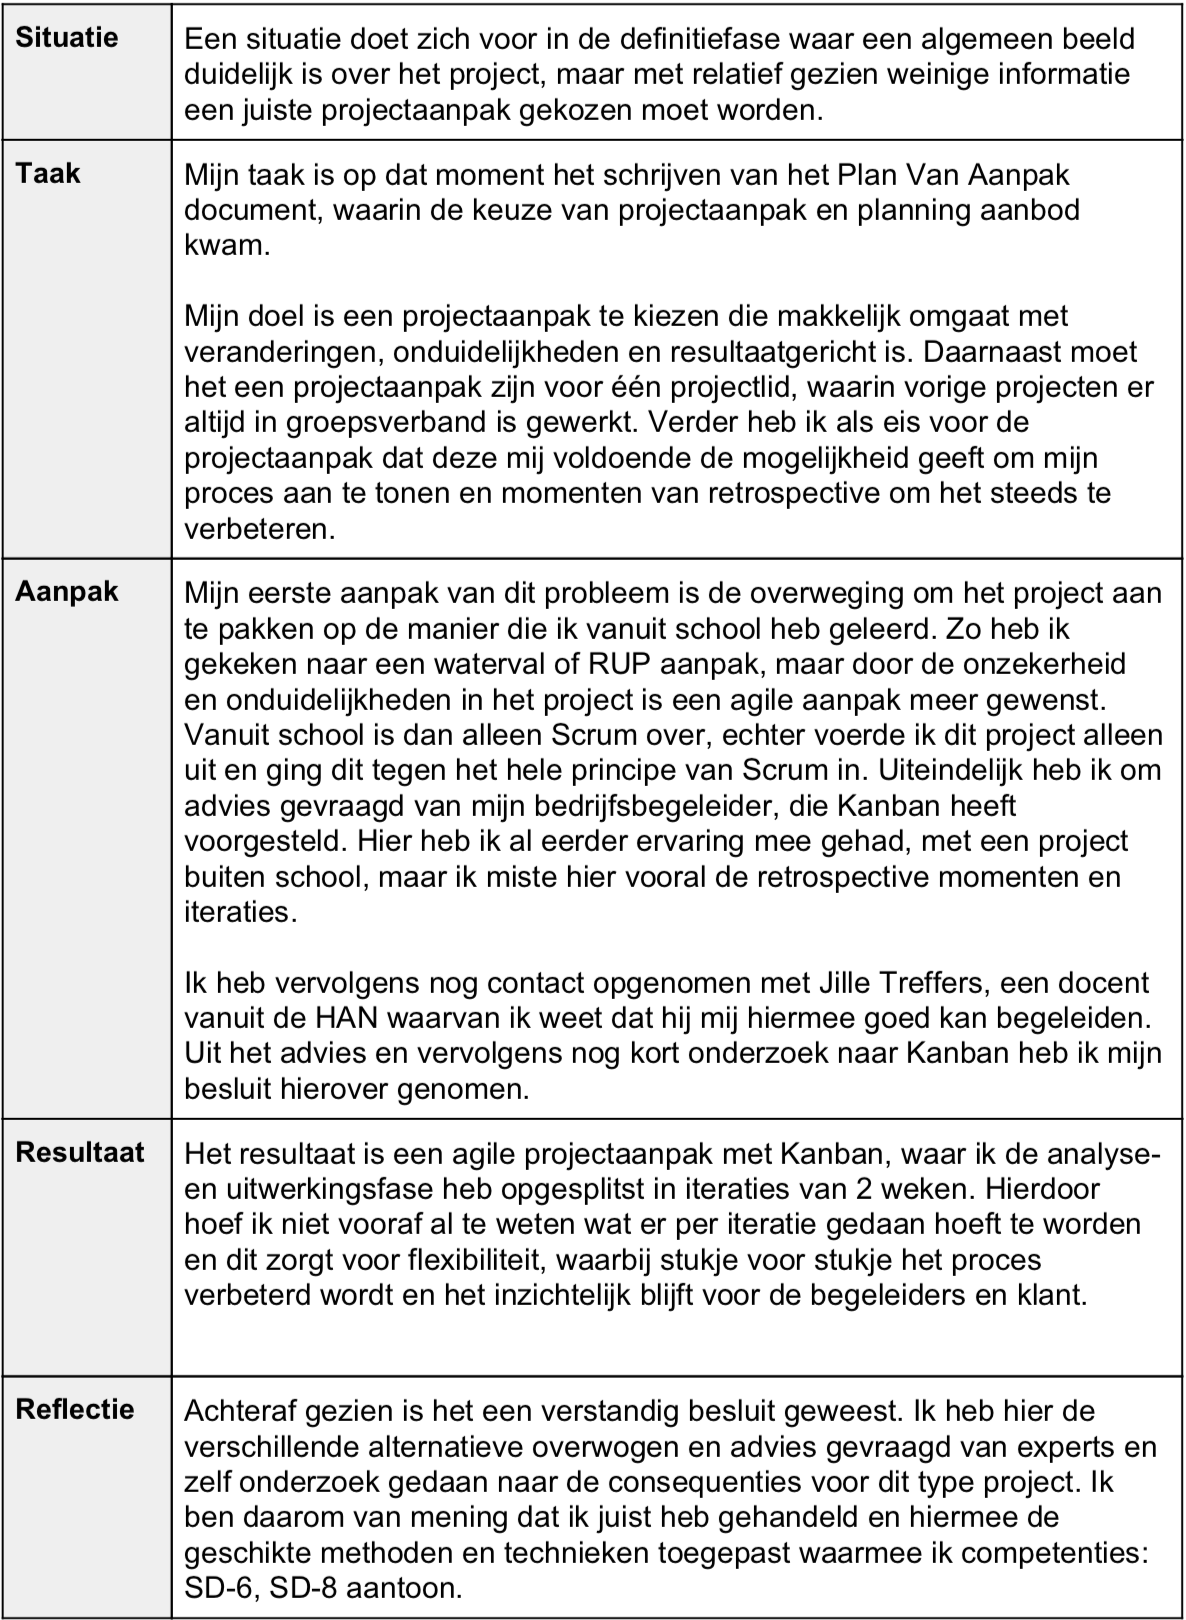
\includegraphics[width=\paperwidth-200]{images/sit_projectaanpak}

\subsection{Communicatie met de opdrachtgever}
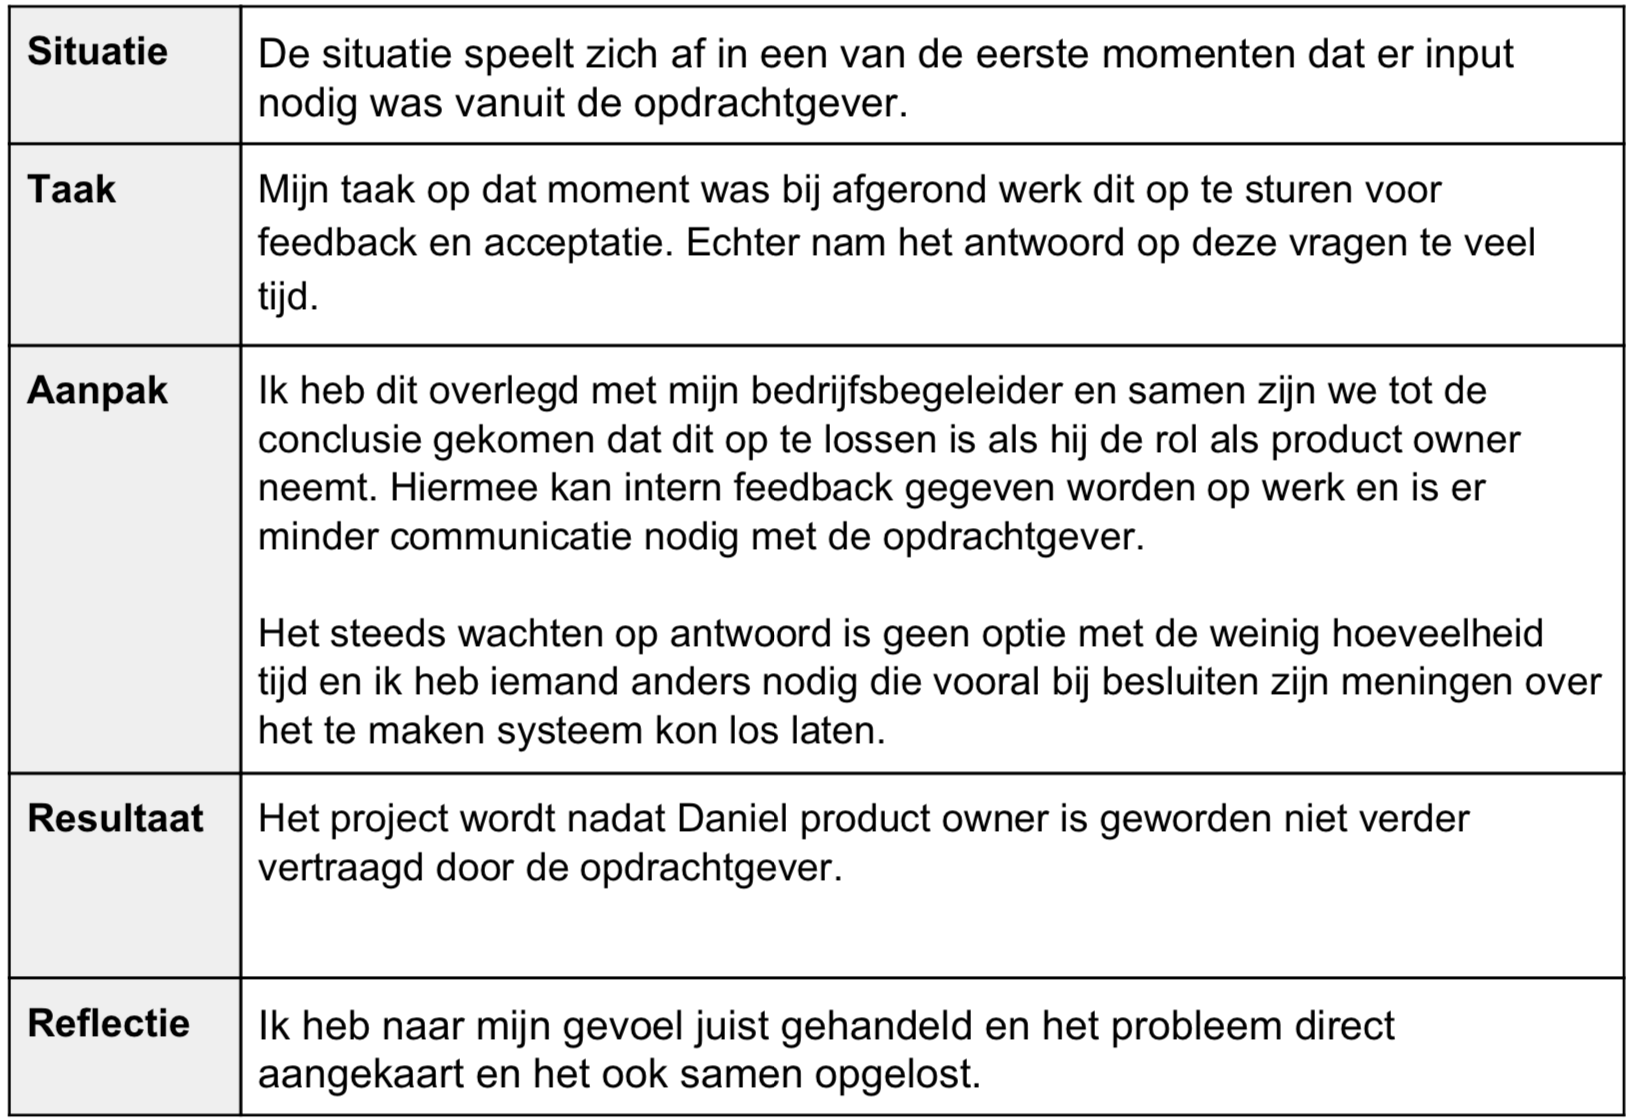
\includegraphics[width=\paperwidth-200]{images/sit_comm}

\subsection{Oplossingsrichtingen planmatig vergelijken}
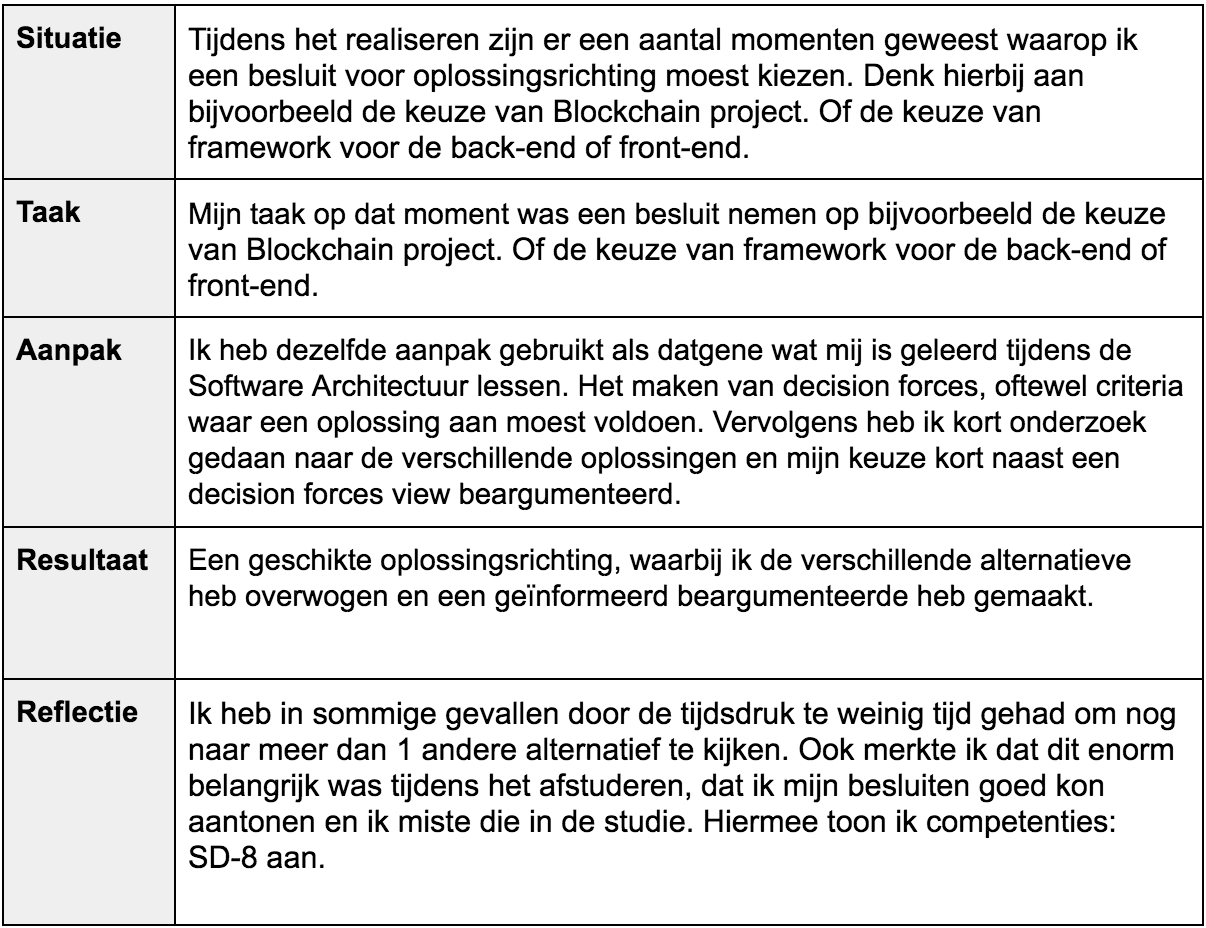
\includegraphics[width=\paperwidth-200]{images/sit_oplossingrichting}

\subsection{Analyse software design documenteren}
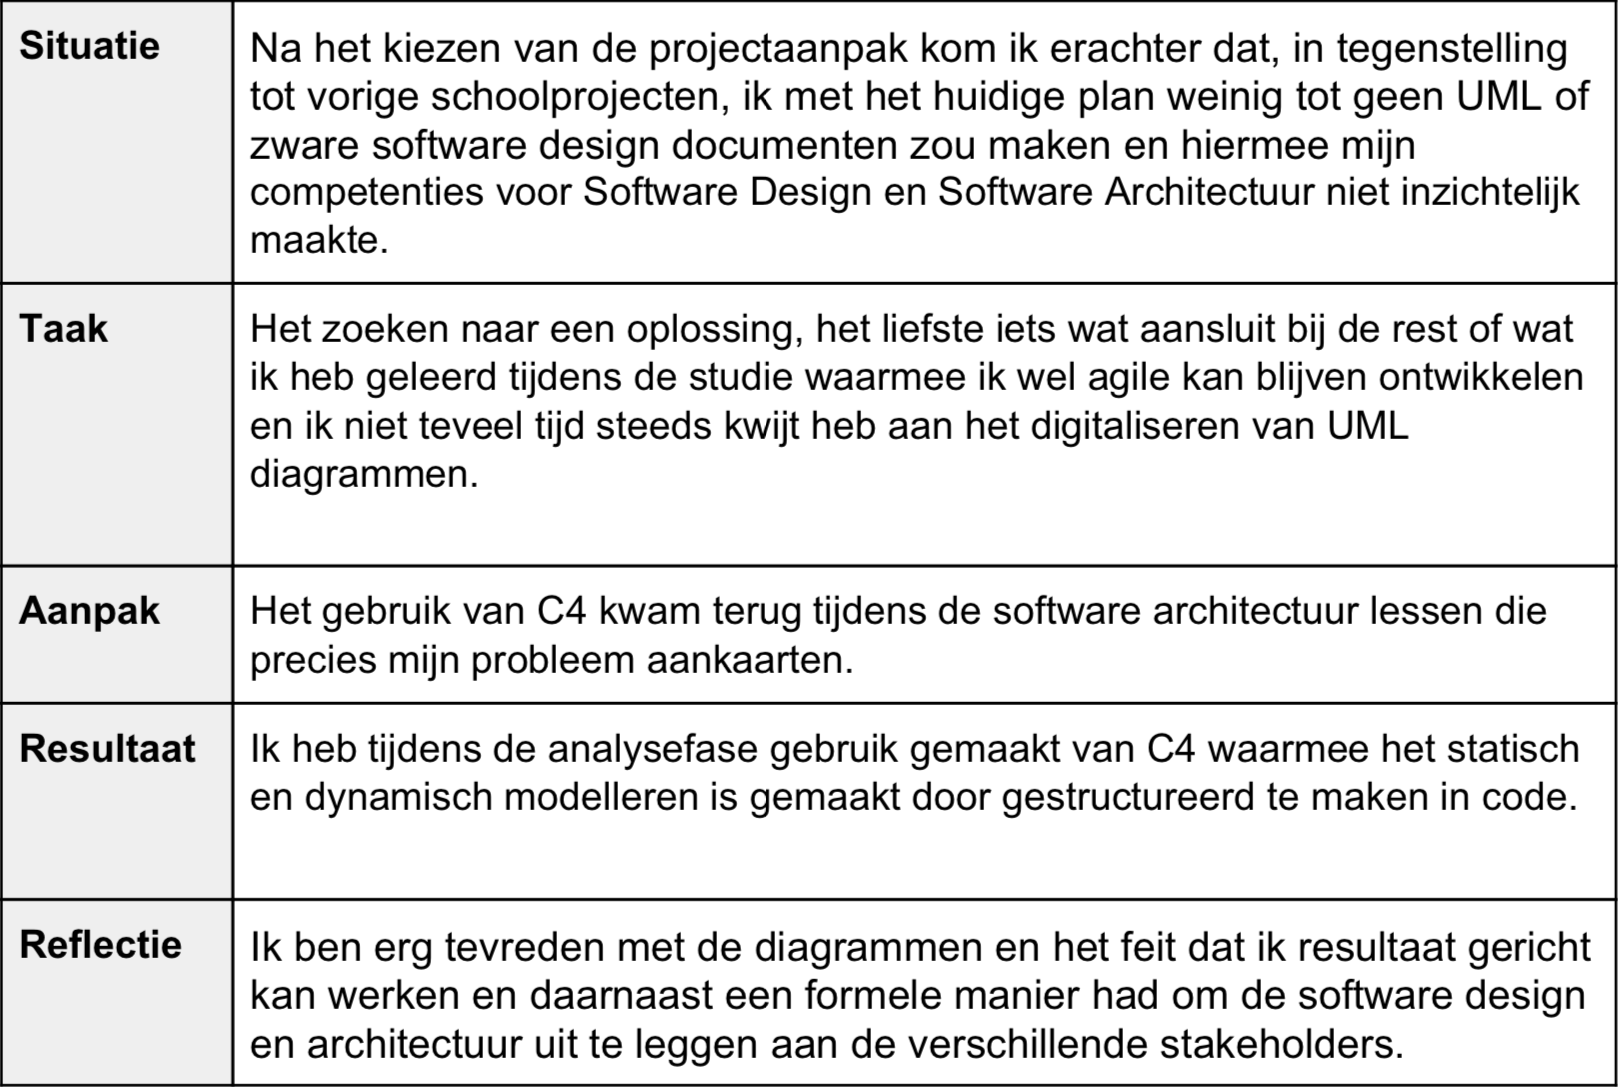
\includegraphics[width=\paperwidth-200]{images/sit_modelana}


%%%%%%%%%%%%%%%%%%%%%%%%%%%%%%%%%%%%%%%%%%%%%%%%%%%%%%%%%%%%%%%%%%%%%%%%%%%%%%
%%
%% Bibliography:
%%
%\cleardoublepage
%\phantomsection
\addcontentsline{toc}{chapter}{Bibliografie}
\bibliography{thesis}

% %%%%%%%%%%%%%%%%%%%%%%%%%%%%%%%%%%%%%%%%%%%%%%%%%%%%%%%%%%%%%%%%%%%%%%%%%%%%%%%%
% %% Appendix:
% %%

%\chapter{Bijlagen}

\end{lstlisting}


%%%%%%%%%%%%%%%%%%%%%%%%%%%%%%%%%%%%%%%%%%%%%%%%%%%%%%%%%%%%%%%%%%%%%%%%%%%%%%%%
%% Index:
%%
% \printthesisindex

\end{document}
